\documentclass[en]{pracamgr}

\usepackage{graphicx}
\usepackage{caption}
\usepackage{subcaption}
\usepackage{amsmath}

\usepackage{etoolbox}
\apptocmd{\thebibliography}{\raggedright}{}{}

\autor{Marcin Papierzyński}{345782}

\title{Music Style Transfer}
\titlepl{Transfer Stylu Muzycznego}

\kierunek{Computer Science}

\opiekun{dr hab. Marek Cygan\\
  Instytut Informatyki
  }

% miesiąc i~rok:
\date{September 2019}

%Podać dziedzinę wg klasyfikacji Socrates-Erasmus:
\dziedzina{11.4 Artificial Intelligence}

%Klasyfikacja tematyczna wedlug AMS (matematyka) lub ACM (informatyka)
\klasyfikacja{Applied computing\\
  Arts and humanities\\
  Sound and music computing}

\keywords{style transfer, music, midi, neural networks}

\newtheorem{defi}{Definicja}[section]

\begin{document}
\maketitle

%tu idzie streszczenie na strone poczatkowa
\begin{abstract}
  TODO
\end{abstract}

\tableofcontents
%\listoffigures
%\listoftables

\chapter{Introduction}

Transfer of style between images is a well-known problem.
Currently it can be realized between any two images by using convolutional neural networks.
The analogous style transfer done for music is a much less explored topic and it is challenging even to define what exactly a musical style is.

In this paper the goal is to define some sensible notion of musical style and create a model that can create a different arrangement for any song based on style extracted from any other song.
The music used for training is assumed to be in the MIDI format and can use any range of instruments.
The instruments supported by the model must be set during training, but the supported styles do not -- we want the trained model to be able to extract style from any song.

\chapter{Other works}

There exist previous works doing music style transfer to some extent.
A few examples are shortly described below.
All of them, however, are performing a simpler kind of a style transfer.

\section{Neural Translation of Musical Style}

In Neural Translation of Musical Style \cite{neural_translation} authors created a model than can learn to perform any given piano piece in either jazz or classical style.
The model does this by regression of notes' velocities (loudness), so it's effectively creating an interpretation of a given piano piece.
Therefore it's much simpler, because it only supports one instrument (piano) and cannot create a completely different arrangement.

\section{Symbolic Music Genre Transfer with CycleGAN}

In Symbolic Music Genre Transfer with CycleGAN \cite{cyclegan} the described model can create new arrangements but it can still only generate piano and the styles need to be set during training (in this case it's jazz, classic and pop).

\section{Play as You Like: Timbre-enhanced Multi-modal Music Style Transfer}

In Timbre-enhanced Multi-modal Music Style Transfer \cite{multimodal} the model can operate on different instruments, but the styles still need to be set during training (the styles are actually instruments, the authors are using guitar, piano and string quartet).
Like in the previous examples, it doesn't allow to transfer style between arbitrary songs.

\chapter{Overview and results}

\section{Musical style and composition}

For musical style transfer, the two main notions concerning songs are composition and style.
I start by giving a rough definition of them.

Composition is any information about a song that is related to a specific moment in time, e.g. if the music gets louder or some instrument starts playing.
The most important part of a composition is the melody (played by one or more instruments).

The style, on the other hand, is information not related to any specific moment in time, e.g. the general mood of the song or the way specific instruments are used (for example, which instruments play the main melodic line and which ones create a backing).

Since music is a form of art, even though it can be understood and formally described, it will always be at least partly subjective.
This means that the exact way to split songs into composition and style is not unique (for example, used instruments may naturally be considered part of style, but they can also change in time).
The main assumption, however, is that composition-style splitting can be performed in \emph{some} fashion which can be learned by a complex enough model.

Since any song can be naturally interpreted as a time sequence, I will use a recurrent neural network as a model for splitting the input song into composition and style.
Composition, just like the input, is a time series, but simpler, with less features.
The style, on the other hand, is a single vector representing the whole song.
During training, the model splits the input song into composition and style, and then combines them to recreate the original song.
Because composition is much smaller than the input song, the model must include useful information in the style vector as well.

After training, I can use the model to extract style from some song and combine it with the composition extracted from other song.
The hypothesis is that this approach will allow for a sensible music style transfer.

\section{Results}

TODO

\chapter{Framework}

\section{Tools}

The whole project is implemented in Python.
The machine learning framework I use is PyTorch, along with mido -- a Python library for working with MIDI files.

\section{Data}

The dataset I use is Lakh MIDI Dataset\footnote{https://colinraffel.com/projects/lmd/}.
It contains over 100,000 songs in the MIDI format and covers various genres, including pop, rock or classical.

\chapter{Data flow}

The data flow of the whole architecture is composed of 3 stages: style extraction, predicting song information, and style application.

\section{Style extraction}

The input in the first stage is:
\begin{itemize}
    \item song information
    \begin{itemize}
        \item instruments used in a song
        \item mode of a song (major or minor)
        \item tempo (in beats per minute)
    \end{itemize}
    \item song content (information about which notes are played in any moment in time for any instrument used in a song)
\end{itemize}

Mode and used instruments are represented using one-hot encoding.
I use 41 most popular instruments in the dataset (percussion and 40 pitched instruments) covering 90\% of all the sounds in the dataset.
The tempo is a numerical value between 50 and 200 (and is clamped to that interval, if necessary).

The output is composed of 3 parts: melody, rhythm and style.
Each of them contains features as learnable embeddings.
I will refer to melody and rhythm as composition.

Melody should encode song content (like the input) but with no information about specific instruments (it must combine them).
It encodes all pitched instruments used in a song.

Rhythm contains additional information about the melody (but not explicitly related to specific notes) and features of percussion if it is present in the input song.
The main reason for introducing rhythm alongside melody is to be able to represent percussion (the only unpitched instrument) but at the same time do not force it if it's not present in the original song (the model should be able to add percussion to a song that originally didn't have it).

I require that there is always at least one pitched instrument used in a song, while the percussion is optional.
That way both melody and rhythm are always well-definied (there is at least one pitched instrument they can encode).

Melody and rhythm, along with the style, should enable to recreate all the instruments used in a song.

\section{Prediction of song information}

The input in this stage is style and rhythm.
The output is basic information about a song (as in the first stage):
\begin{itemize}
    \item used instruments (classification)
    \item mode (classification)
    \item tempo (regression)
\end{itemize}

All those outputs should coincide with the respective inputs from the first stage.
Note that the set of supported instruments can be arbitrarily large but needs to be specified during training.

\section{Style application}

At this stage the inputs are composition (i.e. melody and rhythm) and style from the first stage.
The output is the song content for each of the used instruments.
Generated song content should conincide with the input from the first stage.
In other words, the model must reconstruct the original song.

\chapter{Data representation}

In MIDI format, the song is encoded as a sequence of events messages.
Messages can contain instructions like setting the tempo or playing a note.
Note events are assigned to one of the 16 channels -- each of those channels can represent a different instrument.

\section{MIDI encoding}

The MIDI file is encoded as a tensor in the format:
\begin{center}
    (\emph{batch, channel, bar, beat, beat fraction, note, note features}).
\end{center}

The \emph{channel} dimension refers to a MIDI channel (an instrument).
The \emph{bar}, \emph{beat} and \emph{beat fraction} dimensions point to the exact moment in a song when the note is being played.

\subsection{Specifying time}

I assume that the time signature cannot change, so that the number of the beats is constant throughout the song (usually 3 or 4).
The \emph{bar} and \emph{beat} dimensions denote in which bar and at which beat the note should play.
The \emph{beat fraction} dimension is specifying the exact moment during the beat.

I divide the beat into 8 parts, which gives 8 possible fractions: $0, \frac{1}{8}, \frac{2}{8}, \ldots, \frac{7}{8}$.
Independently, I also divide the beat into 3 parts: $0, \frac{1}{3}, \frac{2}{3}$.
Combining it, symplifying and sorting, we get 10 different fractions:
$$
0, \frac{1}{8}, \frac{1}{4}, \frac{1}{3}, \frac{3}{8}, \frac{1}{2}, \frac{5}{8}, \frac{3}{4}, \frac{2}{3}, \frac{7}{8}.
$$

Each \emph{note fraction} coordinate represents one of those fractions.
A single beat most commonly has length of a quarter note, which means that fractions with denominator 8 allow to represent up to 32th notes.
While division into powers of 2 is the most common in music, many songs also use division into three parts, called triplets.
Inclusion of fractions with denominator 3 allows for the exact representation of them, which otherwise would need to be approximated using fractions with denominator 8.
More fractions could be added to allow for representing faster melodies, but these 10 are enough for most songs.

The typical way of splitting the beat in neural music generation is to simply divide it into timesteps of equal length, e.g. into 12 parts \cite{clara}.
The downside of this approach is that it creates many "unnecessary" fractions (like $\frac{1}{12}$), which are not typically used, so they mainly only increase the size of the MIDI file representation.
The increase in the size is quite significant, since being able to represent 32th notes using this approach would require denominator $24=3\cdot8$, resulting in the whole input being over two times bigger.
Here I only introduce the fractions that are necessary to represent triplets ($\frac{1}{3}$ and $\frac{2}{3}$), omitting the rest.

The proposed approach also scales well with addition of more tuplets.
For example, adding support for quintuplets (division into 5 parts) would only require adding 4 more fractions ($\frac{1}{5}, \frac{2}{5}, \frac{3}{5}$ and $\frac{4}{5}$), resulting in a constant increase in size ($14=10 + 4$ timesteps), while the traditional approach would mean a 5-fold increase in the total size ($120=3\cdot5\cdot8$ timesteps). More complex tuplets are however much less common (and virtually never used in popular music), so I don't use them here.

It's worth noting that in my approach resulting fractions are not equidistant, meaning that it's not justified to apply convolution along the \emph{note fraction} dimension.
However, the length of this dimension is not substantial and it's still possible to apply convolution along \emph{bar} and \emph{beat} dimensions, so it's not a big limitation.

\subsection{Note features}

The above format is used for both percussion and pitched instruments.
However, the number of notes and note features (lengths of dimensions \emph{note} and \emph{note features} respectively) is different for percussion and for pitched instruments, so two tensors must be used: one for pitched instruments and one (possibly empty) for percussion.

Note features for pitched instruments are:
\begin{itemize}
    \item velocity (loudness)
    \item duration
    \item accidentals (raise or lower the note one semitone)
\end{itemize}

For percussion the only note features are velocity and duration.

\section{Notes' representation}

I use note's span of 8 octaves, each with 12 sounds, which gives 96 possible notes in total.
The notes are represented as one-hot encoded vectors with a slight modification.
In the standard one-hot encoding, each coordinate in a \emph{note} dimension would correspond to a specific note (so \emph{note} dimension would have length 96).
However, this way of encoding would pose a problem for style transfer.
Namely, depending on the mode of the song (major or minor), a different set of notes is used.
This means that the same song in a different mode would use different sounds in its melody.
Hence, with the typical way of encoding notes, the melody representation would partially impose style, which is not desired, since we want to split them.

To remedy that, I encode the notes relative to the scale the song is in.
Effectively, what is encoded are not the actual notes, but rather the scale degrees they represent; so the note C in a song in C major would be encoded the same way as the note G in a song in G minor.
That way, changing the scale of the song will not affect the melody representation.

This way of encoding only allows to encode notes contained in a given scale (which covers 7 out of 12 notes in each octave).
For example, if the song is in C major, we could only encode "white keys".
To allow for encoding all the remaining notes as well, each note has additional features (called accidentals) that can raise it or lower it one semitone.
Then we can represent all 12 notes in each octave.

The downside of this solution is that it requires the scale of the song to be known -- and finding it is in itself not a trivial problem.
I use fairly simple heuristics based on the Krumhansl-Schmuckler key-finding algorithm\footnote{http://rnhart.net/articles/key-finding/}, which predicts the scale of the song based on the frequency of notes used.

\section{Style and composition representation}

Melody is a tensor of shape
\begin{center}
    (\emph{batch, channel, bar, beat, beat fraction, note, features}),
\end{center}
which is the same as the input shape but with no \emph{instrument} dimension.
The number of note features may also be different.

Rhythm is a tensor of shape
\begin{center}
    (\emph{batch, channel, bar, beat, beat fraction, features}).
\end{center}
It's also similar to the input but this time with no \emph{instrument} and no \emph{note} dimensions.

Style is encoded as a regular vector, so it has shape
\begin{center}
    (\emph{batch, features}).
\end{center}

The number of features in a melody should be low enough so that the model cannot simply remember all the instruments in the input.
Instead, the model will need to learn some compressed high-level representation of the melody, from which it will later be able to reconstruct the input instruments, using the style vector.

\chapter{Model}

TODO

Convolutions, LSTM.


\chapter{Experiments}

\section{Loss function}

The loss function measures if the song generated by the model is the same as the input song. It is defined as a combination of many components, with the following structure:
\begin{itemize}
    \item total loss
	\begin{itemize}
	    \item channels loss
		\begin{itemize}
			\item pitched channels loss
            \begin{itemize}
                \item notes loss (complement of smooth F1 score)
                \item velocity loss (MSE)
                \item duration loss (MSE)
                \item accidentals loss (cross-entropy)
            \end{itemize}
			\item unpitched channels loss
            \begin{itemize}
                \item notes loss (complement of smooth F1 score)
                \item velocity loss (MSE)
                \item duration loss (MSE)
            \end{itemize}
		\end{itemize}
        \item song information loss
        \begin{itemize}
            \item instruments loss (cross-entropy)
            \item tempo loss (MSE)
            \item mode loss (cross-entropy)
        \end{itemize}
	\end{itemize}
\end{itemize}

This hierarchy signifies that the total loss is the average of channels loss and song information loss, channels loss is the average of pitched and unpitched channels loss, etc.

Notes loss is measuring if the model is generating the right sounds.
Since the desired output is greatly unbalanced (most of all the possible notes will not be played), I'm using a complement of smooth F1 score to measure notes loss:
\nopagebreak

\begin{equation}
    \textrm{notes loss} = 1 - F_1.
\end{equation}

Smooth $F_1$ score is definied in a standard way, using
\nopagebreak
\begin{align}
    & \textrm{true positive} = \min(p, t), \\
    & \textrm{false positive} = \max(0, p - t), \\
    & \textrm{false negative} = \max(0, t - p),
\end{align}

where $p,t\in[0,1]$ are prediction and ground truth respectively, interpreted as fuzzy logical values.
In case when $p$ and $t$ can only take discrete values of 0 or 1, this gives a standard definition of the $F_1$ score.
Thus, it is a generalization of the $F_1$ score compatible with gradient descent.
In our case the notes' fuzzy logical values are defined from velocity (1 meaning that the note is played with maximum possible velocity, and 0 meaning that the note is not played at all).

Velocity loss measures if the model is generating notes with the right loudness.
Velocity is already measured by the notes loss (acquiring maximum $F_1$ score requires playing with exactly right velocities), so this loss function provides additional, more explicit component measuring the velocity error.
It only takes into account the notes that should be played to avoid problems with unbalanced output (the same is true for duration loss).

Since different kinds of loss functions have different magnitudes, before averaging, all the components are normalized to take values in the $[0,1]$ interval.
Then, the normalized components are averaged using quadratic mean to yield the total loss. The use of quadratic mean instead of arithmetic promotes minimizing the components that have the greatest value, resulting in a more balanced training.

\section{Training}

The model was trained for 2000 iterations using the Adam optimizer \cite{adam}.
In each iteration the input is a random song from the dataset. Figure \ref{fig:total} shows total loss during training, while figures \ref{fig:channels} and \ref{fig:song_info} show specific components of the loss function. All the plots are smoothed using exponential moving average with momentum parameter equal to .99 and initial bias equal to 1 (maximum possible error).

\begin{figure}
    \centering
    \begin{subfigure}{.5\linewidth}
        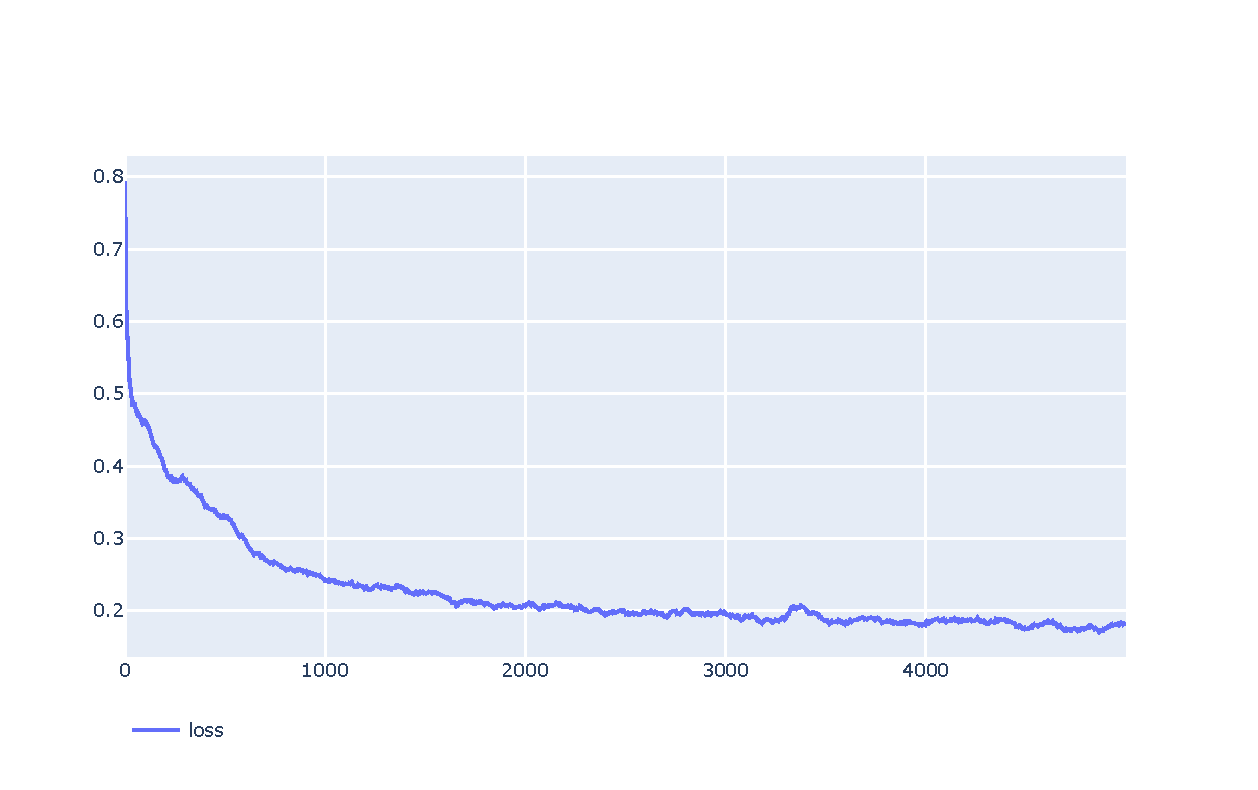
\includegraphics[width=\linewidth]{figures/training.pdf}
        \caption{Total loss.}
    \end{subfigure}%
    \begin{subfigure}{.5\linewidth}
        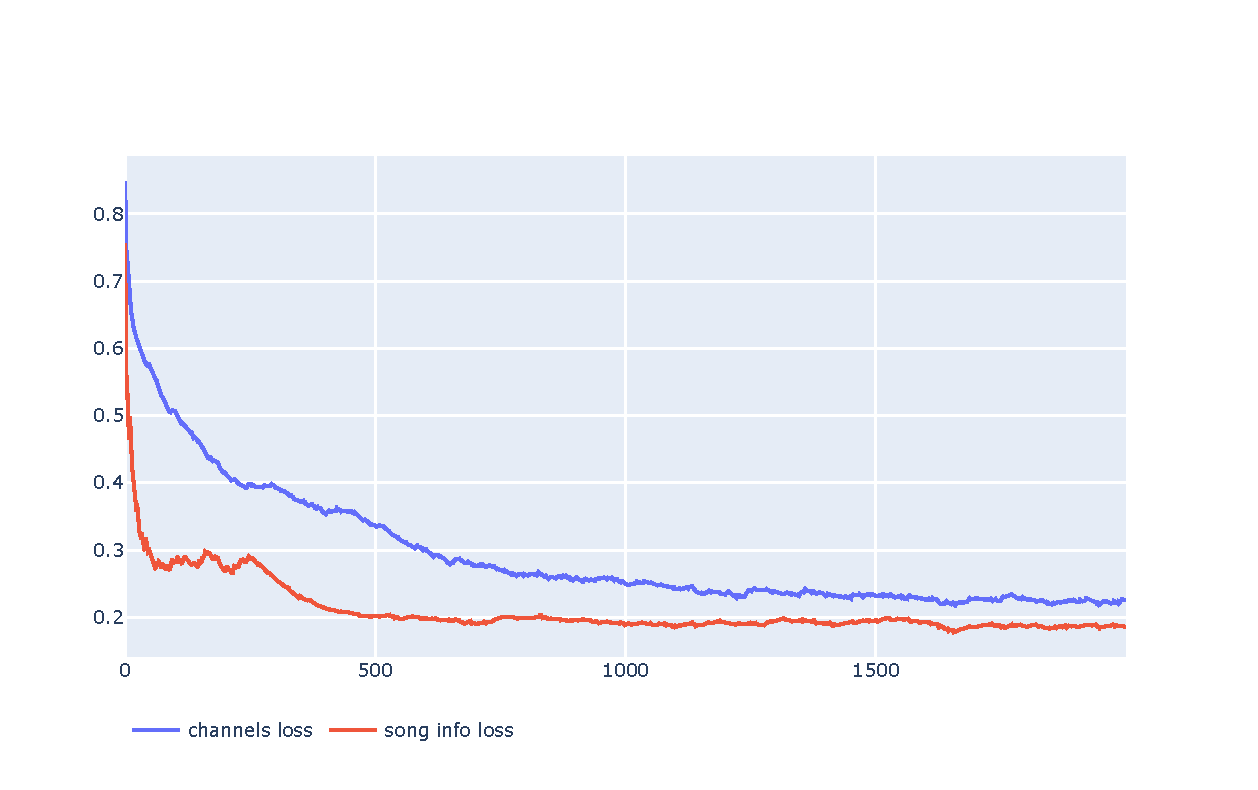
\includegraphics[width=\linewidth]{figures/total.pdf}
        \caption{Loss components.}
    \end{subfigure}%
    \caption{Total loss and its components during training. As can be seen on the second plot, predicting basic song information is easier than generating music, especially at the beginning of training.}
    \label{fig:total}
\end{figure}

Figure \ref{fig:pitched_vs_unptiched} shows how pitched and unpitched notes losses compare during trainig.
In general percussion is easier for the model, as indicated by lower error value for the most time of training.
Interestingly however, approximately during iterations 200-800 the unpitched notes loss is significantly higher (around .7) than the pitched notes loss (around .55).
Possible explanaition is that it's easy to achieve this level of unpitched notes loss by mostly repeating the most common drum patterns.
This hypothesis can be confirmed by listening to the music generated by the snapshot of the model at iteration 300 (before unpitched notes loss started to decrease again).
As it turns out, the generated percussion is indeed very basic, only featuring some typical drum patters found in most of the pop/rock music.
To achieve lower unpitched notes loss the model needed to start encoding some useful information about percussion, but could not do so explicitely per note (like for pitched instruments), which explains why for some time percussion posed a main challenge for the model.

\begin{figure}
    \centering
    \begin{subfigure}{\linewidth}
        \centering
        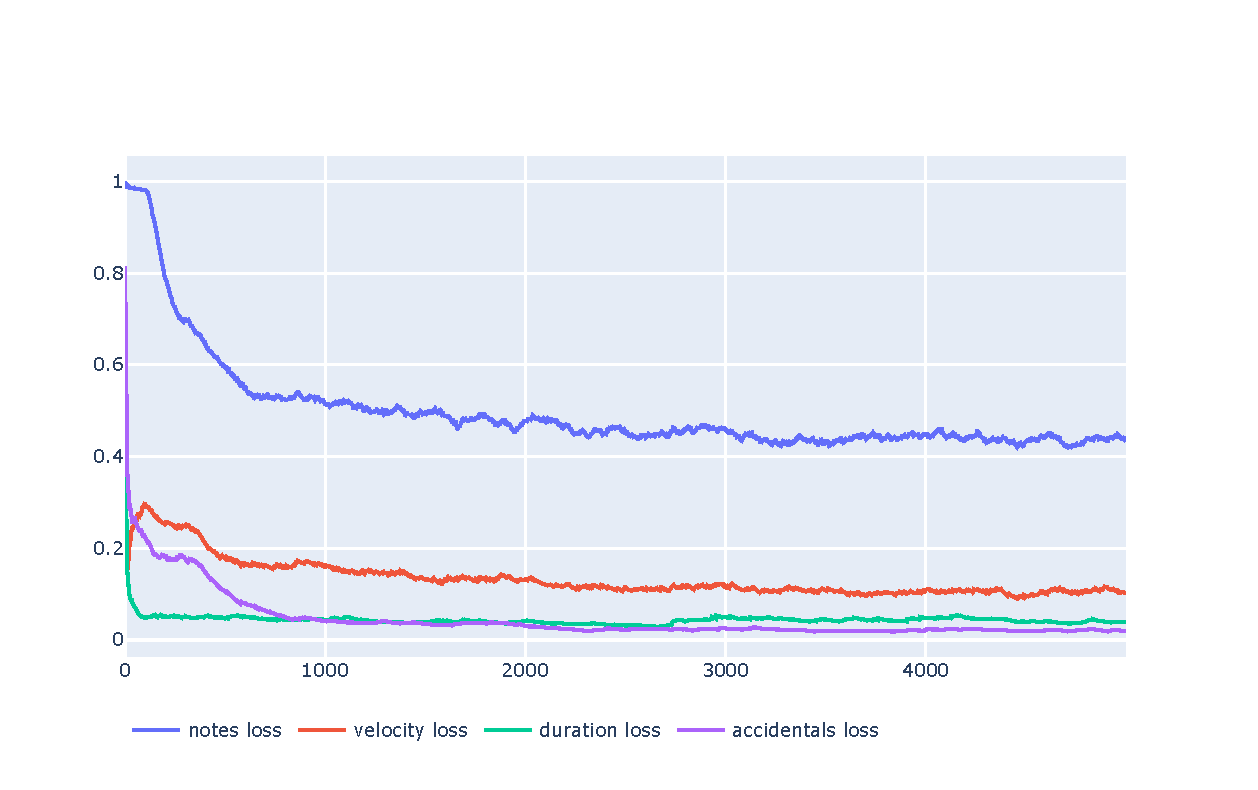
\includegraphics[width=.9\linewidth]{figures/pitched.pdf}
        \caption{Pitched loss components.}
    \end{subfigure}
    \begin{subfigure}{\linewidth}
        \centering
        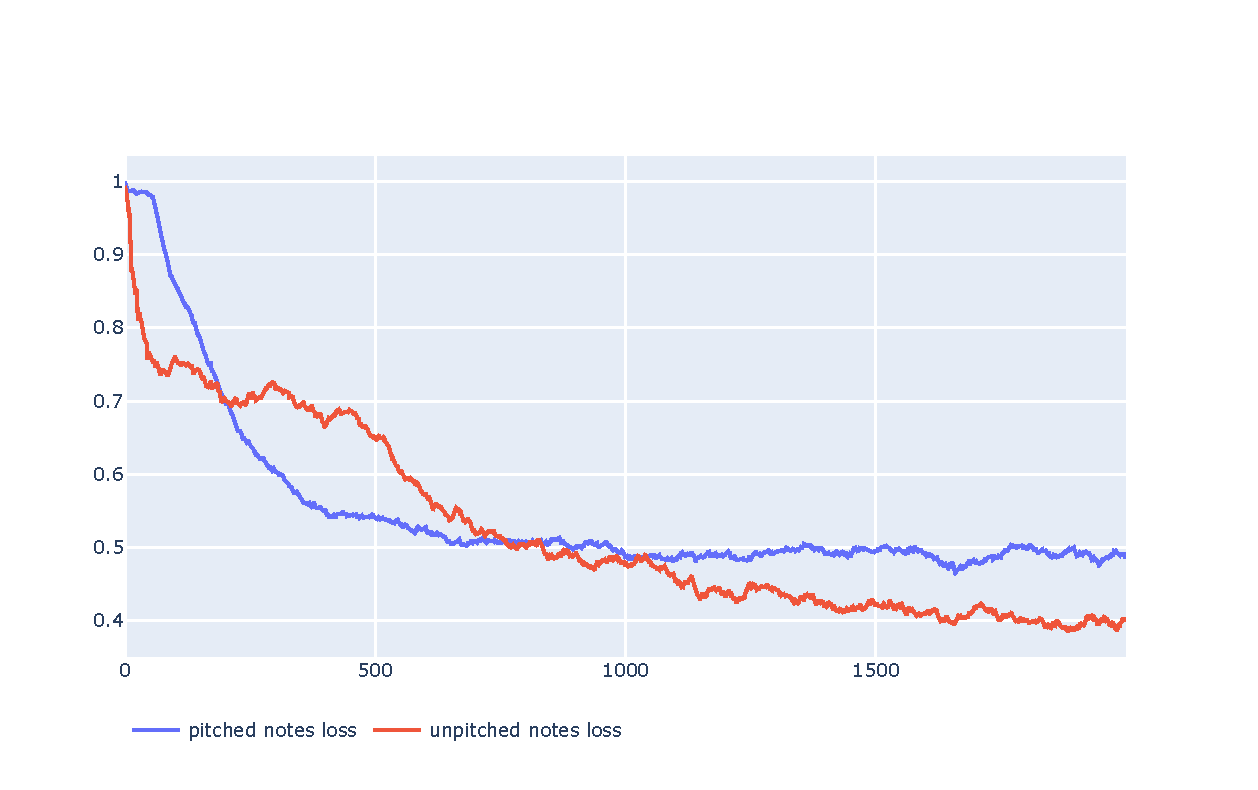
\includegraphics[width=.9\linewidth]{figures/notes.pdf}
        \caption{
            Comparision of pitched and unpitched notes loss.
            The red line represents how well the model is playing the percussion, while the blue line represents all the other instruments.
            We can see that in general pitched instruments are harder than percussion -- at the beginning the model needs some time to start learning to play pitched instruments, and pitched notes loss eventually saturates at higher level than unpitched notes loss.
            There are however a few hundred iterations during training when the model is actually better at playing pitched instruments than percussion.
        }
        \label{fig:pitched_vs_unptiched}
    \end{subfigure}
    \caption{Channels loss during training.}
    \label{fig:channels}
\end{figure}

\begin{figure}
    \centering
    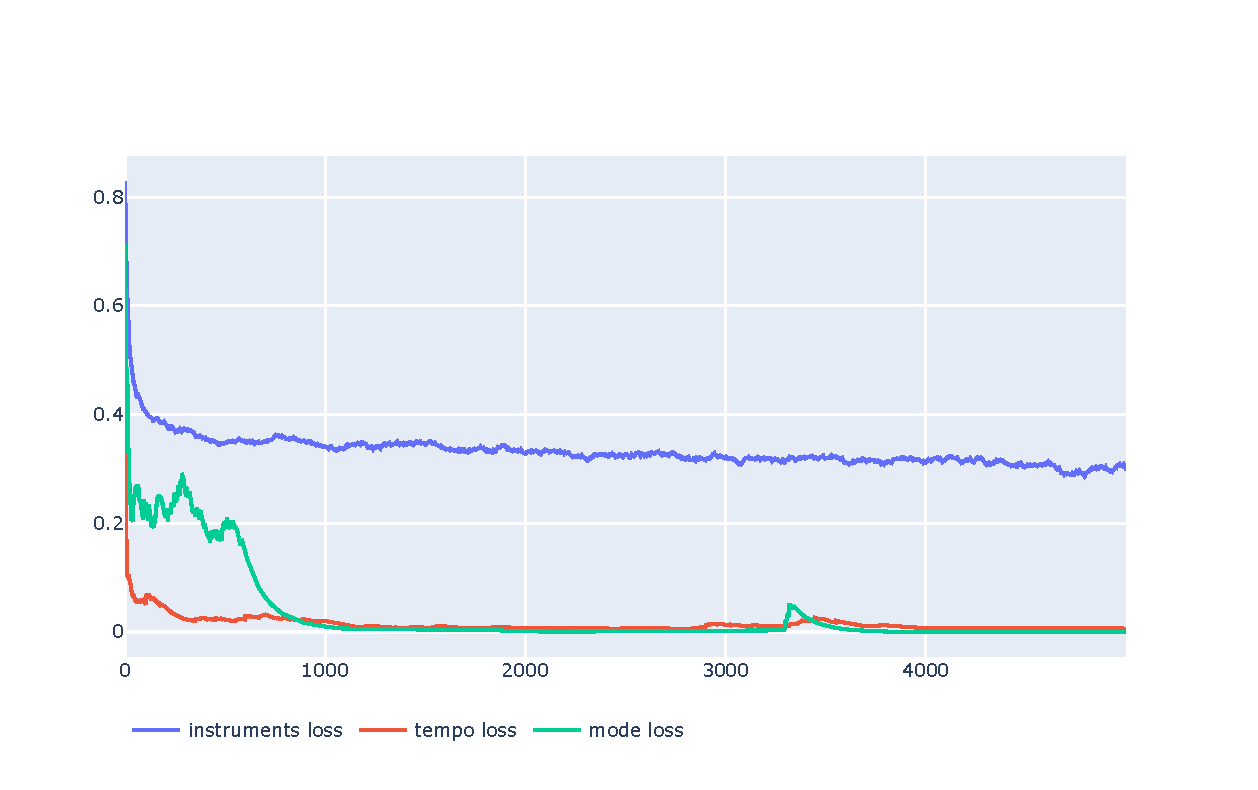
\includegraphics[width=\linewidth]{figures/song-info.pdf}
    \caption{Song information loss components during training.}
    \label{fig:song_info}
\end{figure}

\section{Style transfer}

TODO

After training, the model is used to extract style and composition from two songs and then generate songs from these compositions but with switched styles.

\begin{thebibliography}{99}
\addcontentsline{toc}{chapter}{Bibliography}

\bibitem{neural_translation} Iman Malik, Carl Henrik Ek, \textit{Neural Translation of Musical Style}, https://arxiv.org/abs/1708.03535.

\bibitem{cyclegan} Gino Brunner, Yuyi Wang, Roger Wattenhofer, Sumu Zhao, \textit{Symbolic Music Genre Transfer with CycleGAN}, https://arxiv.org/abs/1809.07575.

\bibitem{multimodal} Chien-Yu Lu, Min-Xin Xue, Chia-Che Chang, Che-Rung Lee, Li Su, \textit{Play as You Like: Timbre-enhanced Multi-modal Music Style Transfer}, https://arxiv.org/abs/1811.12214.

\bibitem{clara} Christine Payne, OpenAI Scholars Program, \textit{Clara: Generating Polyphonic and Multi-Instrument Music Using an AWD-LSTM Architecture}, http://www.christinemcleavey.com/files/clara-musical-lstm.pdf.

\bibitem{adam} Diederik P. Kingma, Jimmy Ba, \textit{Adam: A Method for Stochastic Optimization}, https://arxiv.org/abs/1412.6980.

\end{thebibliography}

\end{document}
